\chapter{Сложный атом}

\section{Вариационный принцип, вычисление энергии основного состояния}

Пусть для системы с гамильтонианом $\op{H}$ задача решена, то есть найдены значения энергии $E_n$ и волновые функции $\Psi_n$, такие что:
$$
\op{H}\Psi_n = E_n \Psi_n,~~ n = 0,1,2...
$$

Волновые функции $\Psi_n$ ортонормированы:
$$
\bk{\Psi_n}{\Psi_m} = \delta_{nm}
$$
и образуют полный базис.

Рассмотрим произвольную пробную волновую функцию $\Phi$, нормированную на единицу:
$$
\bk{\Phi}{\Phi} = 1
$$

Её разложение по базису $\brcr{\Psi_n}$ имеет вид:
$$
\Phi = \sum_n a_n \Psi_n
$$

В силу условий нормировки для коэффициентов $a_n$ имеем:
$$
\sum_n \abs{a_n}^2 = 1
$$

Среднее значение энергии системы с волновой функцией $\Phi$ имеет следующий вид:
\begin{equation}
\label{eq:18_1_1}
\avg{E} \equiv \mathcal{E}[\Phi] \equiv \bfk{\Phi}{\op{H}}{\Phi}  = \sum_n \sum_m \bfk{a_n \Psi_n}{\op{H}}{a_m \Psi_m} = \\ = \sum_n \sum_m a_n^* a_m E_m \delta_{nm} = \sum_n \abs{a_n}^2 E_n
\end{equation}

Здесь значение интеграла зависит от вида функции, поэтому $\avg{E}$ есть <<функция от функции>>, т.е. функционал. Обозначим функционал символом $\mathcal{E}[\Phi]$. Заменяя в сумме \eqref{eq:18_1_1} значения энергий $E_1$, $E_2$, \dots на наименьшее значение $E_0$ --- энергию основного состояния, и поскольку  $E_n \geqslant E_0$ ($n=0, 1, 2, \dots$), получим неравенство:
\begin{equation}
\label{eq:18_1_2}
\boxed{\mathcal{E}[\Phi] \geqslant E_0 \sum_n \abs{a_n}^2 = E_0}
\end{equation}

Это значит, что средние значения энергии, вычисленные с пробными функциями $\Phi$, являются оценками сверху для точной энергии основного состояния. При $\Phi = \Psi_0$ следует, что $\mathcal{E}[\Psi_0] = E_0$.
Поэтому задача определения собственной функции $\Psi_0$ основного состояния может быть сформулирована так: из всех допустимых (т.е. однозначных, непрерывных и нормированных) функций найти такую, для которой среднее значение энергии $\mathcal{E}[\Phi]$ минимально:
%(\autoref{fig:18_1}).
\begin{equation}
\label{eq:18_1_3}
\mathcal{E}[\Phi] \to \min
\end{equation}

%\begin{figure}[h!]
%\centering
%\begin{tikzpicture}[domain=-1.5:1.5]
%  \draw[->] (0,-2) -- (0,1) node[above] {$E$};
%  \draw[-] (-0.1,0) -- (0.1, 0) node[right] {$0$};
%  \draw[-] (-0.1,-1) -- (0.1,-1) node[right] {$\mathcal{E}[\Phi]$};
%  \draw[-] (-0.1,-1.5) -- (0.1, -1.5) node[right] {$E_0$};
%\end{tikzpicture}
%\caption{Соотношение между энергиями.} \label{fig:18_1}
%\end{figure}

Исследование экстремальных значений функционалов типа $\mathcal{E}[\Phi]$ проводится методами вариационного исчисления; при этом требование \eqref{eq:18_1_3} для $\mathcal{E}[\Phi]$ формулируется следующим образом: вариация $\delta \mathcal{E}$ должна обращаться в нуль
\begin{equation}
\label{eq:18_1_4}
\delta \mathcal{E} = 0
\end{equation}
для всех допустимых вариаций $\delta\Phi$ функции $\Phi$, удовлетворяющей дополнительному условию $\bk{\Phi}{\Phi} = 1$.

Ниже предполагается следующий алгоритм поиска волновой функции $\Phi$ основного состояния:
\begin{enumerate}
\item выбираем пробную функция, зависящую от координат $q$ и ряда параметров $\alpha_i$ (вариационных параметров):
$$
\Phi = \Phi(q, \alpha_1, \alpha_2 ... );
$$
\item вычисляем среднюю энергию в состоянии, описываемом данной функцией:
$$
\bfk{\Phi}{\op{H}}{\Phi} = \mathcal{E}(\alpha_1, \alpha_2 ...);
$$
\item минимизируя $E$ по параметрам $\alpha_i$:
$$
\pd{\mathcal{E}}{\alpha_1} = 0,~~ \pd{\mathcal{E}}{\alpha_2} = 0, \dots
$$
находим те значения параметров $\alpha_i^0$, для которых $\mathcal{E}$ минимально.
\end{enumerate}

После выполнения описанной выше процедуры можно утверждать, что функция $\Phi(q, \alpha_1^0, \alpha_2^0, \alpha_2^0, \dots)$ есть наилучшее приближение к $\Psi_0(q)$ в выбранном классе функций. Этот метод поиска наилучшего приближения к $\Psi_0(q)$ называют вариационным.

Следует отметить, что вычисления поправок к уровням энергии электронов He в первом порядке теории возмущений, что проводилось в \S 2 главы \rom{17}, эквивалентны вычислениям с помощью вариационного метода при не лучшем выборе пробной функции. В предыдущей главе в нулевом приближении мы получили для координатной волновой функции основного состояния атома He следующее выражение:

\begin{equation}
\label{eq:18_1_5}
\Phi_{g.s}^{S}(\vr_1, \vr_2) = \phi_{1s}(\vr_1)\phi_{1s}(\vr_2) = \frac{1}{\pi} \brc{\frac{Z}{a}}^3 e^{-\frac{Z(r_1 + r_2)}{a}}
\end{equation}

Кулоновское отталкивание электронов в атоме He можно учесть более удачным выбором волновой функции нулевого приближения. Каждый электрон частично экранирует заряд ядра для другого электрона. Поэтому они движутся в поле с некоторым эффективным зарядом $\tilde{Z} < Z = 2$. Следовательно, волновую функцию основного состояния атома He можно искать в виде
\begin{equation}
\label{eq:18_1_6}
\Phi_{g.s}(\vr_1, \vr_2) = C e^{-\frac{\tilde{Z}(r_1 + r_2)}{a}},
\end{equation}
где $\tilde{Z}$ --- вариационный параметр, а постоянная $C$ определяется условием нормировки. Вычисляя среднюю энергию как функцию $\tilde{Z}$,
$$
\bfk{\Phi_{g.s}^{S}}{\op{H}}{\Phi_{g.s}^{S}} = \mathcal{E}(\tilde{Z}),
$$
и затем минимизируя $\mathcal{E}(\tilde{Z})$: $\pd{\mathcal{E}}{\tilde{Z}} = 0$, находим:
$$
\tilde{Z} = Z - \frac{5}{16}
$$

Можно улучшить оценку для энергии основного состояния атома He, увеличивая число варьируемых параметров.

\section{Метод Хартри-Фока. Приближения центрального поля. Электронные конфигурации}

Перейдем к общему случаю сложного атома, имеющего $N$ электронов и заряд ядра $-Ze$ ($e<0$). Нерелятивистский гамильтониан такого атома имеет вид:
\begin{equation}
\label{eq:18_2_1}
\op{H} = \sum_{i=1}^{N} \brc{\frac{\op{\vp_i}^2}{2m} - \frac{Ze^2}{r_i}} + \sum_{i<j} \frac{e^2}{\abs{\vr_i - \vr_j}}
\end{equation}

$N$-электронная задача не имеет точных решений, т.е. из-за последней суммы в выражении \eqref{eq:18_2_1} нет разделения переменных, описывающих пространственное движение электронов. На примере атомов He мы видели, что каждый электрон фактически движется поле, создаваемом ядром и другим электроном, т.е. в некотором эффективном среднем (по движению другого электрона) поле. Физическим и математическим обобщением идеи эффективного среднего поля для описания движения выделенного $i$-го электрона в $N$-электронной системе является метод Хартри-Фока (1928-1930 гг.). Метод исходит из функционала электронной энергии
\begin{equation}
\label{eq:18_2_2}
\mathcal{E}\brs{\{\psi_{\{n_j\}}(\xi_i)\}} = \bfk{\Uppsi^{HF}}{\op{H}}{\Uppsi^{HF}}
\end{equation}
построенного для гамильтониана \eqref{eq:18_2_1} на хартри-фоковской волновой функции $N$-электронной системы $\Uppsi^{HF}(\xi_1, \xi_2, \dots, \xi_N)$, взятой в виде детерминанта Слэтера \eqref{eq:16_2_2} (приближение Хартри было модифицировано в 1930 г. В.А. Фоком так, чтобы полная волновая функция $N$ электронов имела правильную симметрию относительно их перестановки). В результате поиска наилучших одноэлектронных конфигураций $\psi_{\{n_j\}}(\xi_i)$ (спин-орбиталей), т.е. минимизирующих функционал энергии \eqref{eq:18_2_2}, приходят к системе из $N$ связанных между собой интегро-дифференциальных уравнений для спин-орбиталей. Систему уравнений называют уравнениями Хартри-Фока. С точки зрения физического смысла каждое из уравнений Хартри-Фока описывает движение выделенного $i$-го электрона в некотором среднем эффективном поле $U_{cc}(\vr_i)$, созданном ядром и остальными электронами атома. 

%\item 
%$$
%\mathcal{E}\brs{\{\psi_{\{n_j\}}(\xi_i)\}} = \min~ \forall \delta\psi_{\{n_j\}}(\xi_i)
%$$
%\end{enumerate}

Это поле $U_{cc}(\vr_i)$ является центральным и самосогласованным, т.к. оно зависит от электронного состояния атома, которое, в свою очередь, зависит от $U_{cc}(\vr_i)$ (приближение центрального самосогласованного поля). В приближении центрального поля гамильтониан \eqref{eq:18_2_1} можно представить в виде
\begin{equation}
\label{eq:18_2_3}
\op{H} = \underbrace{\sum_{i=1}^{N} \brc{\frac{\op{\vp_i}^2}{2m} + U_{cc}(\vr_i)}}_{\op{H}^{(0)}} + \op{V},
\end{equation}
где нецентральная часть
$$
\op{V} = \sum_{i<j} \frac{e^2}{\abs{\vr_i - \vr_j}} + \sum_{i=1}^N \brc{-\frac{Ze^2}{r_i} - U_{cc}(\vr_i)}
$$
описывает остаточное кулоновское взаимодействие в атоме.

Асимптотика самосогласованного поля обладает сферической симметрией: $U_{cc}(\vr_i) = U_{cc}(r_i)$ и имеет следующий вид:
$$
U_{cc}(r_i) =
\begin{cases}
-\dfrac{Ze^2}{r_i},& r_i \to 0\\
-\dfrac{(Z-(N-1))e^2}{r_i},& r_i \to \infty\\
\end{cases}
$$

Такой потенциал отличен от кулоновского (в различных асимптотиках числитель изменяется), поэтому уровни энергии электрона в сложном атоме, в отличие от водородоподобного атома, зависят от $n$ и $l$ $\to E_{nl}$, то есть в сложном атоме снимается вырождение по $l$. В качестве одночастичного базиса для $\op{H}^\zr$ следует выбрать состояния электрона в центрально-симметричном поле, т.е.
$$
\psi_{\{n_j\}}(\xi_i) = R_{n_j l_j}(r_i) Y_{l_j m_j}(\theta_i, \phi_i) \chi_{\frac{1}{2} \lambda_j}(\sigma_i)
$$

В соответствии с этими результатами электроны в сложном атоме распределяются по одночастичным состояниям $\ket{n~l~m_l~m_s}$, каждое из которых характеризуется главным квантовым числом $n$, орбитальным $l$, магнитным квантовым числом $m_l$ и проекцией ($m_s = \pm \dfrac{1}{2}$) $\lambda$ спина на ось $z$. Основному состоянию атома отвечает минимальная энергия, поэтому электроны заполняют одночастичные состояния последовательно, начиная с самых глубоких.

\begin{defn}
Совокупность состояний с заданными $n$ и $l$ называется \underline{электронной оболочкой} атома.
\end{defn}
Такая совокупность содержит $2(2l + 1)$ состояний.

\begin{defn}
Электроны, находящиеся в состояниях с одинаковыми $n$ и $l$, называются \underline{эквивалентными}.
\end{defn}

Главное квантовое число указывается цифрой перед буквенными обозначениями орбитального момента $l$. Число эквивалентных электронов указывается в виде верхнего индекса у обозначения оболочки. Например, основное состояние атома He обозначается $1s^2$, а первое возбужденное состояние есть $1s^12s^1$.

\begin{defn}
Распределение электронов по оболочкам называется \underline{электронной конфигурацией}. 
\end{defn}

Оболочка, содержащая $2(2l + 1)$ электронов называется заполненной. При суммировании по всем состояниям заполненной оболочки получаем:
\begin{gather*}
M_L = \sum_{i = 1}^{2(2l+1)} m_{l_i} = 2 \sum_{m_l=-l}^{+l} m_l = 0, \\ 
M_S = \sum_{i = 1}^{2(2l+1)} m_{s_i} \\
\end{gather*}

Поскольку суммарная проекция орбитального момента (спинового момента) единственное значение, равное нулю, то суммарный орбитальный момент и суммарный спиновые момент заполненной оболочки равны нулю: $L=0$, $S=0$.

Следовательно, операторы полного орбитального момента и полного спина всех электронов атома
\begin{equation}
\label{eq:18_2_4}
\op{\vec{L}} = \sum_{i = 1}^{N} \op{\vec{l}}_i,~~~\op{\vec{S}} = \sum_{i = 1}^{N} \op{\vec{s}}_i
\end{equation}
реально формируются только из операторов $\op{\vec{l}}_i$, $\op{\vec{s}}_i$ электронов незаполненной оболочки.

\section{Интегралы движения в сложных атомах. Термы. Правила Хунда}

Можно показать, что операторы $\op{\vec{L}}$ и $\op{\vec{S}}$ коммутируют с гамильтонианом $\op{H}$ \eqref{eq:18_2_1} атома. Поэтому может быть построена общая система собственных векторов операторов  $\op{H}$, $\op{\vec{L}}^2$, $\op{L_z}$, $\op{\vec{S}}^2$ и $\op{S_z}$. Каждый такой собственный вектор $\ket{L M_L S M_S}$ определяет состояние атома с энергией $E$.

Если в последней $(nl)$ оболочке имеются $k < 2(2l+1)$ электронов (оболочка не заполнена), то говорят, что состояние атома описывается электронной конфигурацией $nl^k$. При этом, как показало исследование атома He, энергии состояний зависят от суммарного спина $S$ электронов (см. \eqref{eq:17_2_6}). Кроме того, в предыдущем параграфе было показано, что уровни энергии электрона в сложном атоме зависят еще и от $l$, а значит, электронная энергия сложного атома зависит не только от $S$, но и от $L$:
$$
E = E(S, L) = \bfk{L M_L S M_S}{\op{H}}{L M_L S M_S}
$$ 

Уровни энергии атома принято называть \underline{термами} и ставить им в соответствие спектроскопические символы:
$$\boxed{^{2s+1}L},$$
где число $2s+1$ называют мультиплетностью терма.

Каждый терм вырожден $(2S+1)(2L+1)$ раз (по квантовым числам $M_S$ и $M_L$). Поэтому орбитальному моменту $L$ так же, как и орбитальному моменту $l$ отдельного электрона, ставят в соответствие заглавные латинские буквы так, как это делалось для атома водорода (\S 5 главы \rom{8}):
$$ 
\begin{matrix}
L= & 0, & 1, & 2,& 3, & \dots \\
      & S, & P, & D, & F, & \dots 
\end{matrix}
$$

Введем полный угловой момент электронной оболочки атома:
\begin{equation}
\label{eq:18_3_1}
\op{\vec{J}} = \op{\vec{L}} + \op{\vec{S}},
\end{equation}
где по правилу сложения моментов \eqref{eq:15_2_4} число $J$ при заданных $L$ и $S$ пробегает диапазон значений:
$$
J = \abs{L-S}, \abs{L-S} + 1, ..., L+S
$$

Получаем новый набор коммутирующих операторов $\op{H}^{SO}$, $\op{\vec{L}}^2$, $\op{\vec{S}}^2$,$\op{\vec{J}}^2$ и $\op{J_z}$ с учетом того, что теперь в оператор $\op{H}^{SO}$ входит еще оператор спин-орбитального взаимодействия $\op{V}^{SO} = A \vec{L} \cdot \vec{S}$, т.е. $\op{H}^{SO} = \left .\op{H} \right |_{\eqref{eq:18_2_1}} + \op{V}^{SO}$. В присутствии $\op{V}^{SO}$ операторы $\op{L_z}$ и $\op{S_z}$ не коммутируют с гамильтонианом $\op{H}^{SO}$ атома и поэтому уже не являются интегралами движения.

\begin{excr}
Доказать, что $[\op{V}^{SO}, \op{L_z}] \neq 0$ и $[\op{V}^{SO}, \op{S_z}] \neq 0$.
\end{excr}

Прежний набор квантовых чисел, $L M_L S M_S$, теперь непригоден для характеристики состояния атома с учетом спин-орбитального взаимодействия, и необходимо перейти к другому набору: $J M_J L S$. В итоге уровни энергии атома в новом представлении характеризуются термом 
$$
\boxed{^{2s+1}L_J}
$$
%Для проекции полного момента верно:
%$$
%\op{J}_z = \op{L}_z + \op{S}_z
%$$


Для каких значений $J$, $L$ и $S$ уровень атома будет иметь минимальное значение энергии? Ответ на этот вопрос дают эмпирические \underline{правила Хунда} (1925 г.):
\begin{enumerate}
\item Для заданной электронной конфигурации наименьшей энергией обладает терм с наибольшим возможным значением $S$ и наибольшим (возможным при этом $S$) значением $L$.
\item Минимальную энергию имеет терм с $J = \abs{L-S}$, если заполнено не более половины электронной оболочки, и с $J = L + S$ в противном случае.
\end{enumerate}

\section{$LS$-связь. Тонкая структура уровней. Правило интервалов Ланде}

Рассмотренную выше схему сложения моментов \eqref{eq:18_2_4} и \eqref{eq:18_3_1} в атоме называют $LS$-связью  или связью Рассела-Саундреса (1925 г.). Классификация электронных состояний атомов в случае $LS$-связи в виде спектроскопического символа $^{2s+1}L_J$ справедлива для атомов верхней части таблицы Менделеева, когда спин-орбитальное взаимодействие можно рассматривать как возмущение по сравнению с остаточным кулоновским взаимодействием, описываемым в \eqref{eq:18_2_3} оператором $\op{V}$, т.е. при выполнении условия
\begin{equation}
\label{eq:18_4_1}
\abs{V_{SO}} \ll \Delta E_T,
\end{equation}
когда расстояние между соседними термами существенно превышает разность между компонентами тонкой структуры каждого из термов.
 
Для атомов тяжелых элементов становится существенным релятивистский характер движения электронов ($\dfrac{v_{\text{ат}}}{c} \sim \dfrac{\hbar}{m a c} \sim \dfrac{e^2}{\hbar c} Z = \alpha Z$), когда спиновые и орбитальные переменные в одноэлектронном приближении не разделяются, и приближение $LS$-связи становится неприменимым.
%Эти эффекты становятся существенны около никеля ($Z = 28$).

С учетом оператора спин-орбитального взаимодействия $\op{V}^{SO} = A \op{\vec{L}} \cdot \op{\vec{S}}$ каждый терм расщепится на группу уровней или, как говорят, формируется тонкая структура уровней терма. $(2S + 1)(2L+1)$-кратно вырожденный уровень энергии атома $^{2s+1}L$ расщепится на $2S+1$ уровень, если в сложении моментов \eqref{eq:18_3_1} $L > S$ и на $2L+1$ уровень при $S > L$. 

Возведя операторное равенство \eqref{eq:18_3_1} в квадрат, получим:
$$
\op{\vec{J}}^2 = \op{\vec{L}}^2 + \op{\vec{S}}^2 + 2\op{\vec{L}}\op{\vec{S}}
$$

Значит, оператор спин-орбитального взаимодействия можно представить в виде:
\begin{equation}
\label{eq:18_4_2}
\op{V}^{SO} = A\frac{\op{\vec{J}}^2 - \op{\vec{L}}^2 - \op{\vec{S}}^2}{2}
\end{equation}

Легко видеть, что оператор \eqref{eq:18_4_2} диагонален в базисе $\{ J M_J L S\}$. Поэтому каждое из состояний $\ket{J M_J L S}$ сдвигается на энергию (поправку первого порядка ТВ к энергии $E$):
$$
\Delta E_J = \bfk{J M_J L S}{\op{V}^{SO}}{J M_J L S} = A \frac{J(J+1) - L(L+1) - S(S+1)}{2}
$$

Эта поправка зависит от $J$, но не зависит от $M_J$, т.е. кратность вырождения уровня с полным угловым моментом $J$ равна $2J+1$.

Разность энергий соседних уровней в тонкой структуре терма равна
\begin{equation}
\label{eq:18_4_3}
\Delta E_{J,L,S} - \Delta E_{J-1, L, S} = \frac{A}{2}\brcr{J(J+1) - J(J-1)} = AJ
\end{equation}

Соотношение \eqref{eq:18_4_3} называется \underline{правилом интервалов Ланде} (1923 г.). Уровни, на которые расщепляется атомный терм при учете спин-орбитального взаимодействия, называются компонентами тонкой структуры атомных уровней.

\section{Гамильтониан сложного атома во внешнем магнитном поле}

Рассмотрим атом в однородном и постоянном магнитном поле $\Hvec$. Это магнитное поле может быть описано векторным потенциалом
$$
\vA(\vr) = \frac{1}{2}[\vec{\Hvec} \times \vr],
$$
с кулоновской калибровкой $\Div \vA(\vr) = 0$.

Гамильтониан Паули $i$-го электрона имеет вид \eqref{eq:14_3_8}:
\begin{equation}
\label{eq:18_5_1}
\op{H}(i) = \frac{1}{2m}\brc{\op{\vp}_i - \frac{e}{c}\vA_i}^2 - \frac{e\hbar}{mc}\brc{\op{\vec{s}}_i \cdot \Hvec} + U(\vr_i),
\end{equation}
где $\vA_i = \vA(\vr_i)$, $\mu_B = -\frac{e\hbar}{2mc}$ --- магнетон Бора ($e < 0$), $U(\vr_i) = e\Phi(\vr_i)$ включает в себя все кулоновские взаимодействия, которые входят в гамильтониан \eqref{eq:18_2_1} свободного сложного атома.

Преобразуя первое слагаемое гамильтониана, находим:
\begin{gather*}
\brc{\op{\vp}_i - \frac{e}{c}\vA_i}^2 = \op{\vp}_i^2 - \frac{e}{c}\brc{\op{\vp}_i \vA_i + \vA_i \op{\vp}_i} + \frac{e^2}{c^2}\vA_i^2 
\end{gather*}

Здесь
$$
\op{\vp}_i \vA_i = -i\hbar \nabla_i \vA(\vr_i) + \vA_i \op{\vp}_i,
$$
и т.к. $\Div \vA = 0$, то
\begin{gather*}
\brc{\op{\vp}_i - \frac{e}{c}\vA_i}^2 = \op{\vp}_i^2 - \frac{e}{c}\brc{\op{\vp}_i \vA_i + \vA_i \op{\vp}_i} + \frac{e^2}{c^2}\vA_i^2 = \op{\vp}_i^2 - 2\frac{e}{c}\vA_i \op{\vp}_i + \frac{e^2}{c^2}\vA_i^2 = \\
= \op{\vp}_i^2 - \frac{e}{c}\brc{[\Hvec \times \vr_i], \op{\vp}_i} + \frac{e^2}{c^2}\vA_i^2 = \op{\vp}_i^2 - \frac{e\hbar}{c}(\op{\vec{l}}_i, \Hvec) + \frac{e^2}{c^2}\vA_i^2
\end{gather*}

%Теперь преобразуем второе слагаемое:
%$$
%2\frac{e}{c}\vA_i \op{\vp}_i = 2\frac{e}{c} \frac{1}{2}([\Hvec \times \vr_i], \op{\vp}_i) = \frac{e}{c}%([\op{\vr}_i \times \op{\vp}_i], \Hvec) =\frac{e}{c}(\hbar \op{\vec{l}}_i, \Hvec)   
%$$

%\begin{gather*}
%\op{\vp}_i^2 - 2\frac{e}{c}\vA_i \op{\vp}_i + \frac{e^2}{c^2}\vA_i^2 = \op{\vp}_i^2 - \frac{e\hbar}{c}%(\op{\vec{l}}_i, \Hvec) + \frac{e^2}{c^2}\vA_i^2
%\end{gather*}

Таким образом, гамильтониан атома в магнитном поле с учетом оператора спин-орбитального взаимодействия $\op{V}^{SO}$ выглядит следующим образом:
\begin{gather}
\label{eq:18_5_2}
\op{H} = \sum_{i=1}^N \op{H}(i) + \op{V}^{SO} =  \nonumber \\
= \sum_{i=1}^N \left ( {\frac{\op{\vp}_i^2}{2m} \underbrace{-\frac{e\hbar}{2mc}}_{\mu_B}(\op{\vec{l}}_i \cdot \Hvec) + \frac{e^2}{2mc^2}\vA_i^2 \underbrace{-\frac{e\hbar}{mc}}_{2\mu_B}\brc{\op{\vec{s}}_i \cdot \Hvec}} + U(\vr_i) \right ) + \op{V}^{SO} =  \nonumber \\ 
= \op{H_0} + \op{V}_Z +\op{V}_D,
\end{gather}
где $\op{H}_0 = \sum_{i=1}^N \brc{\dfrac{\op{\vp}_i^2}{2m}  + U(\vr_i)} + \op{V}^{SO}$ --- гамильтониан свободного атома; $\op{V}_Z = \mu_B (\op{\vec{L}} + 2\op{\vec{S}})\cdot \Hvec$ --- оператор зеемановского взаимодействия с внешним магнитным полем электронного момента атома с оператором $\op{\bm{\mu}}_{\text{ат}}$:
$$
\op{V}_Z = -\op{\bm{\mu}}_{\text{ат}} \cdot \Hvec, \text{, т.е.  } \op{\bm{\mu}}_{\text{ат}} = -\mu_B (\op{\vec{L}} + 2\op{\vec{S}});
$$

$\op{V}_D = \dfrac{e^2}{2mc^2} \sum_{i=1}^N \vA_i^2 = \dfrac{e^2}{8mc^2} \sum_{i=1}^N [\Hvec \times \vr_i]^2$ --- оператор диамагнитного взаимодействия.

Пусть $\Hvec = (0, 0, \mathscr{H})$, тогда $\op{V}_Z = \mu_B (\op{{L}}_z + 2\op{{S}}_z) \mathscr{H}$
\begin{equation}
\label{eq:18_5_3}
\op{H} = \op{H}_0 + \mu_B (\op{{L}}_z + 2\op{{S}}_z) \mathscr{H} +\frac{e^2 \mathscr{H}^2}{8mc^2} \sum_{i=1}^N [\vec{n}_z \times \vr_i]^2 
\end{equation}

Квадратичным по $\mathscr{H}$ членом в \eqref{eq:18_5_3} можно пренебречь по сравнению с линейным членом, если
$$
\frac{e^2 \mathscr{H}^2}{mc^2}a^2 \ll \frac{e\hbar}{mc}\mathscr{H}
$$
$$
\mathscr{H} \ll \brc{\frac{e}{a^2}} \brc{\frac{\hbar c}{e^2}} = \mathscr{E}_{\text{ат}} \alpha^{-1} = \mathscr{H}_{\text{ат}} \sim 10^9 \text{ Гс},
$$
где $\alpha = \dfrac{e^2}{\hbar c} \approx \dfrac{1}{137}$ --- постоянная тонкой структуры, $\mathscr{H}_{\text{ат}}$ --- характерное внутриатомное магнитное поле. Таким образом,
\begin{equation}
\label{eq:18_5_4}
\op{H} = \op{H}_0 + \mu_B (\op{L}_z + 2\op{S}_z)\mathscr{H} = \op{H}_0 - \op{\bm{\mu}}_{\text{ат}z} \cdot \Hvec
\end{equation} 

\section{Эффекты Зеемана и Пашена-Бака}

\subsection{Слабое поле}

Магнитное поле называется слабым, если энергия взаимодействия магнитного момента атома с внешним магнитным полем мала по сравнению с интервалами тонкой структуры уровней атома:
\begin{equation}
\label{eq:18_6_1}
\boxed{\abs{V_{\mu_{\text{ат}}\Hsc}} \ll \abs{E_J - E_{J-1}}}
\end{equation}

Напомним, что каждый уровень тонкой структуры обладает энергией
$$
E_J = E + \Delta E_J,
$$
которая складывается из энергии терма $E=E(L, S)$ и сдвига $\Delta E_J$, обусловленного спин-орбитальным взаимодействием $\op{V}^{SO}$ (см. \S 4 этой главы). В отсутствии магнитного поля каждый уровень тонкой структуры $2J + 1$-кратно вырожден по квантовому числу $M_J$. В магнитном поле уровни тонкой структуры расщепляются (эффект Зеемана).

В качестве волновых функций нулевого приближения необходимо использовать базис $\{ \ket{J M_J L S}\}$, в котором в \S 4 решалась задача об интервалах тонкой структуры атома при $\Hvec = 0$. В базисе $\{ \ket{J M_J L S}\}$ сохраняются $\op{\vec{L}}^2$, $\op{\vec{S}}^2$, но не сохраняются $\op{\vec{L}}$ и $\op{\vec{S}}$ в силу их взаимодействия. Зато сохраняется <<вектор>> $\op{\vec{J}}$ --- единственный сохраняющийся <<вектор>> в этом случае.

Векторная схема $\ket{J M_J L S}$-представления показана на \autoref{fig:18_1}. Имеет место прецессия векторов $\vec{L}$ и $\vec{S}$ вокруг сохраняющегося вектора $\vec{J} = \vec{L} + \vec{S}$, причем быстрая по сравнению с прецессией вектора $\vec{J}$ в магнитном поле $\Hvec$, т.к. поле --- слабое в меру неравенства \eqref{eq:18_6_1}, которое эквивалентно
\begin{equation}
\label{eq:18_6_2}
\Omega \ll \omega_{LS},
\end{equation}
где $\Omega$ --- ларморовская частота прецессии $\vec{J}$ в магнитном поле $\Hvec$. %\Omega = \frac{\mu_B \Hsc}{\hbar}$.

\begin{figure}[h!]
\centering
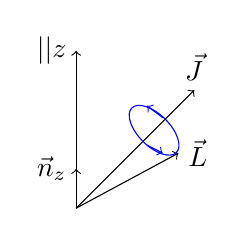
\begin{tikzpicture}[domain=-2:2]
  \draw[->] (0, 0) -- (0, 2) node[left] {$\Hvec || z$};
  \draw[->] (0, 0) -- (0, 0.5) node[left] {$\vec{n}_z$};  
  \draw[->] (0, 0) -- (1.5,1.5) node[above] {$\vec{J}$};
  \draw[->] (0, 0) -- (1.3,0.7) node[right] {$\vec{L}$};
  \draw[rotate=45, blue] (1.4, 0) ellipse (2mm and 4 mm); 
  \draw[blue, ->] (1.1, 1.15) -- (0.9,1.3) ;
  \draw[blue, ->] (0.9, 0.8 ) -- (1.1,0.7) ;

\end{tikzpicture}
\caption{К выводу эффекта Зеемана в слабом поле.} \label{fig:18_1}
\end{figure}

Тогда в первом порядке теории возмущений энергия электронов атома равна 
$$
E_{\Hsc} = E^\zr + \Delta E_{\Hsc}^\one,
$$
где 
$$
\Delta E_{\Hsc}^\one = \mu_B \bfk{J M_J L S}{\underbrace{\op{L}_z + 2\op{S}_z}_{\op{J}_z + \op{S}_z}}{J M_J L S} \Hsc = \mu_B \bfk{J M_J L S}{\op{J}_z + \op{S}_z}{J M_J L S} \Hsc
$$

В базисе $\{ \ket{J M_J L S}\}$
$$
\bfk{J M_J L S}{\op{J}_z + \op{S}_z}{J M_J L S} = g\bfk{J M_J L S}{\op{J}_z}{J M_J L S},
$$
где $g$ --- фактор Ланде. Это утверждение доказывается строго с помощью теоремы Вигнера-Эккарта, мы же этого делать не будем, т.к. достаточно заметить, что это утверждение эквивалентно тому, что
$$
\op{J}_z + \op{S}_z = g\op{J}_z
$$

Последнее равенство уже вполне объяснимо, т.к. $z$-компоненту любого <<вектора>> $\op{\vec{A}}$ можно представить через таковую компоненту единственного сохраняющегося в системе <<вектора>> $\op{\vec{J}}$. Из $[\op{J}_z, \op{A}_z] = 0$ и следует, что 
$$
\op{A}_z = \op{J}_z + \op{S}_z = g\op{J}_z
$$

Найдем $g$-фактор.
\begin{gather*}
\op{J}_z = \op{\vec{J}} \vec{n}_z, \\
\op{S}_z = \op{\vec{S}} \vec{n}_z,
\end{gather*}
тогда
$$
\brc{\op{\vec{J}} + \op{\vec{S}}}\vec{n}_z = \op{J}_z + \op{S}_z = g \op{J}_z = g \op{J}_z = g \op{\vec{J}} \vec{n}_z,
$$
т.е. $\op{\vec{J}} + \op{\vec{S}} = g\op{\vec{J}}$, что тоже можно понять из векторной схемы сложения с неравенством \eqref{eq:18_6_2}. Отсюда
$\op{\vec{J}}^2 + \op{\vec{J}} \op{\vec{S}} = g \op{\vec{J}}^2$ или для квантовых средних $\bfk{J M_J L S}{\op{\vec{J}}^2 + \op{\vec{J}} \op{\vec{S}}}{J M_J L S} = g \bfk{J M_J L S}{\op{\vec{J}}^2}{J M_J L S}$

В базисе $\{ \ket{J M_J L S}\}$ имеем: \newline
$$\avg{\op{\vec{J}}^2} = J(J+1)$$
и из $\op{\vec{J}} - \op{\vec{S}} = \op{\vec{L}}$
$$
\avg{\op{\vec{J}} \op{\vec{S}}} = \frac{1}{2}[J(J+1) + S(S+1) - L(L + 1)]
$$

\begin{equation}
\label{eq:18_6_3}
\boxed{g = 1 + \frac{J(J+1) + S(S + 1) - L(L + 1)}{2J(J+1)}}
\end{equation}

Следовательно,
\begin{equation}
\label{eq:18_6_4}
\Delta E_{\Hsc}^\one = \mu_B g \bfk{J M_J L S}{\op{J}_z}{J M_J L S} \Hsc = \boxed{\mu_B g M_J \Hsc = \Delta E_{\Hsc}^\one}
\end{equation}

При заданном $J$: $M_J = -J, -J + 1, ..., J$, т.е. $\Delta E_{\Hsc}^\one$ принимает $2J+1$ значение. Иными словами, магнитное поле полностью снимает вырождение уровней по направлениям момента $\op{\vec{J}}$ (см. \autoref{fig:18_2}).

\begin{figure}[h!]
\centering
\begin{tikzpicture}[domain=-5:5]
  \foreach \x in {-1.2, -0.8, -0.4, 0, 0.4, 0.8, 1.2}
    \draw[-] (1,\x) -- (2,\x) ;
  \node at (1.5, 2) {$\Hvec \neq 0$};
  \node at (-0.5, 2) {$\Hvec = 0$};
  \draw[-] (-1,0) -- (0,0) ;
  \draw[<->] (1.9, -0.8) -- (1.9,-0.4) node[right] {$\mu_B g \Hsc M_J$};
  \draw[-] (4, 1.8) -- (3.8, 1.8);
  \draw[-] (4, -1.8) -- (3.8, -1.8);
  \draw[-] (4, 1.8) -- (4, -1.8);
  \node [right] at (4, 0) {$2J+1$};
\end{tikzpicture}
\caption{Аномальный эффект Зеемана.} \label{fig:18_2}
\end{figure}

Интервалы между расщепленными подуровнями определяются фактором $\mu_B g(J) \Hsc$, т.е. эти интервалы, вообще говоря, различны для уровней тонкой структуры с разными $J$. Чтобы подчеркнуть удивительность этого результата, говорят об \underline{аномальном эффекте Зеемана}. Если по каким-либо причинам $g(J) = 1$, так что интервалы между состояниями равны $\mu_B \Hsc$, то эффект Зеемана называют \underline{нормальным}.

Эффект Зеемана был обнаружен при сравнении спектров излучения атомов в свободном состоянии и при наличии поля $\Hvec$. Если энергия электронов в атоме до излучения равна $E_1 = E_1^\zr + \mu_B g_1 M_{J_1} \Hsc$, а после излучения равна $E_2 = E_2^\zr + \mu_B g_2 M_{J_2} \Hsc$, то спектр излучаемых частот дается соотношением
\begin{equation}
\label{eq:18_6_5}
\hbar \omega = E_1 - E_2 = (E_1^\zr -E_2^\zr)  + \mu_B \Hsc (g_1 M_{J_1} - g_2 M_{J_2})
\end{equation}

Спектр становится сложным (в формулу \eqref{eq:18_6_5} входят также разные факторы Ланде). Среди частот оптических переходов в атоме, даваемых соотношением \eqref{eq:18_6_5}, экспериментально наблюдаются лишь частоты квантовых переходов, разрешенных \underline{правилами отбора} (см. [4] \S 20.3):
$$
\boxed{\Delta L = 0, \pm 1;~~~ \Delta S = 0; ~~~\Delta J = 0, \pm 1; ~~~ \Delta M_J = 0, \pm 1 }
$$

\subsection{Сильное поле}

Рассмотрим теперь случай сильного поля, когда
$$
\abs{E_J - E_{J-1}} \ll \abs{V_{\mu_{\text{ат}}\Hsc}}  \ll \Delta E_T
$$
%где $\Delta E_T$ - расстояние между соседними термами.

Тогда при увеличении магнитного поля имеет место переход сложного эффекта Зеемана в простой (нормальный) эффект Зеемана или эффект Пашена-Бака (1912 г.).

В этом случае спин-орбитальным взаимодействием можно пренебречь, тогда уже сохраняются <<векторы>> $\op{\vec{L}}$ и $\op{\vec{S}}$, а стало быть, сохраняются и их проекции $M_L$ и $M_S$ на направление поля (ось $z$). Задачу надо решать в базисе $\{ \ket{L M_L S M_S}\}$. С учетом \eqref{eq:18_5_4} имеем:
%Ограничение сверху связано с тем, что наши выкладки верны, пока в атоме сохраняется $LS$-связь.
$$
\Delta E_{\Hsc}^\one = \mu_B \bfk{L M_L S M_S}{\op{L}_z + 2 \op{S}_z}{L M_L S M_S} \Hsc
$$
\begin{equation}
\label{eq:18_6_6}
\Delta E_{\Hsc}^\one = \mu_B \Hsc(M_L + 2 M_S),
\end{equation}
где $M_L = -L, -L + 1, ..., L$; $M_S = -S, -S + 1, ..., S$.

Таким образом, согласно \eqref{eq:18_6_6} в общем случае вырождение атомных уровней энергии с кратностью $(2L+1)(2S+1)$ снимается сильным магнитным полем лишь частично: остается комбинаторика перестановок значений проекций орбитального момента и полного спина при заданном значении $M_L + 2 M_S$. Невырожденными являются низшее и высшее состояния. Спектр наблюдаемых частот: 
\begin{equation}
\label{eq:18_6_7}
\hbar \omega = E_1 - E_2 = (E_1^\zr -E_2^\zr)  + \mu_B \Hsc (\Delta M_L + 2\Delta M_S)
\end{equation}
ограничен правилами отбора (см. [4] \S 20.3):
$$
\boxed{\Delta L = 0, \pm 1;~~~ \Delta S = 0; ~~~\Delta M_L = 0, \pm 1; ~~~ \Delta M_S = 0}
$$